\subsection{\texorpdfstring{Modeling of the QCD Background and $\Wmn$ Signal Yield}{Modeling of the QCD Background the W->mu nu Signal Yield}}
\label{sec:Wmunu}

The $\Wmn$ analysis is performed using fixed distributions for the $\MET$ shapes
obtained from data for the QCD background component and from simulations,
after applying proper corrections, for the signal and the remaining background components.

Different approaches to signal extraction are considered for $\Wmn$, as for $\Wen$.
The alternative methods do not demonstrate better performance than the use of fixed shapes
in the W signal fit. Given the lower backgrounds in the muon channel with respect to the
electron channel, the alternative strategies are not pursued at the same level of detail
as in the electron case.

The $\MET$ shape of the QCD background component is obtained from a high-purity QCD sample
of events that pass the signal selection, except that the isolation requirement
is inverted and set to $\IRelComb > 0.2$ (Fig.~\ref{figure:Wmunu_iso}).

Simulation studies indicate that this distribution does not accurately
reproduce the $\MET$ shape when muon isolation is required.
This is shown in Fig.~\ref{figure:Wmunu_QCD} (left),
where the solid line represents the shape for events with an isolated muon and the dashed line
the shape obtained by inverting the isolation requirement. %They are very distinct.

A positive correlation between the isolation variable $\IRelComb$ and $\MET$ is shown
in Fig.~\ref{figure:Wmunu_QCD} (right, red open circles). This behavior can be
parameterized in terms of a linear function
$\MET\propto (1+\alpha\,\IRelComb)$, as shown in the same figure.
A compensation for the correlation is subsequently made
by applying a correction of $\MET^\prime = \MET/(1+\alpha\,\IRelComb)$ to
the events selected by inverting the isolation requirement and a new corrected shape is obtained.
The agreement of this new shape (black points in Fig.~\ref{figure:Wmunu_QCD}, left)
with the prediction from events with an isolated muon is considerably improved.
It is also observed that a maximal variation in the correction factor of $\Delta \alpha =  0.08$ successfully
covers the simulation prediction for events with an isolated muon over the whole $\MET$ interval (shaded area in Fig.~\ref{figure:Wmunu_QCD}, left).
\begin{figure}[htbp] {\centering
    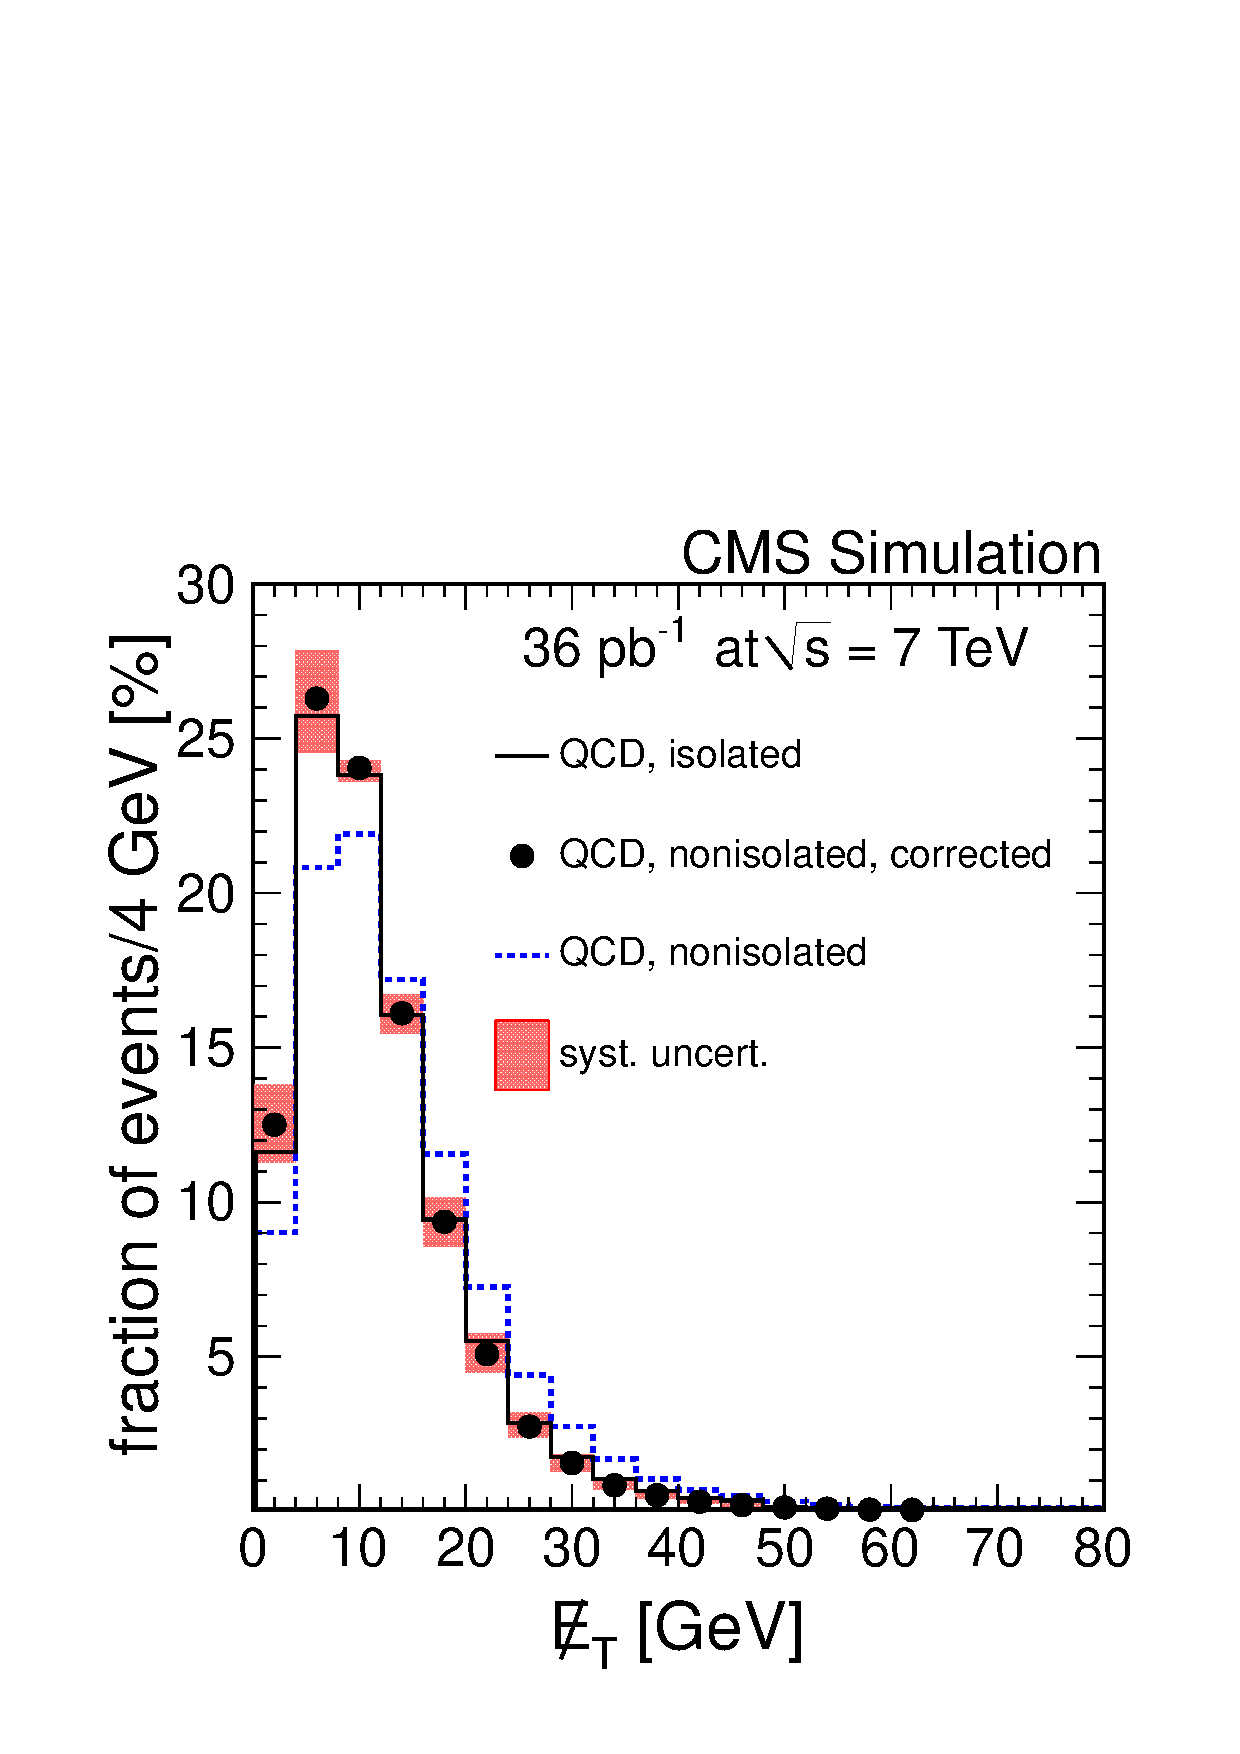
\includegraphics[width=7.5cm]{figs/qcd_template_MC.pdf}
    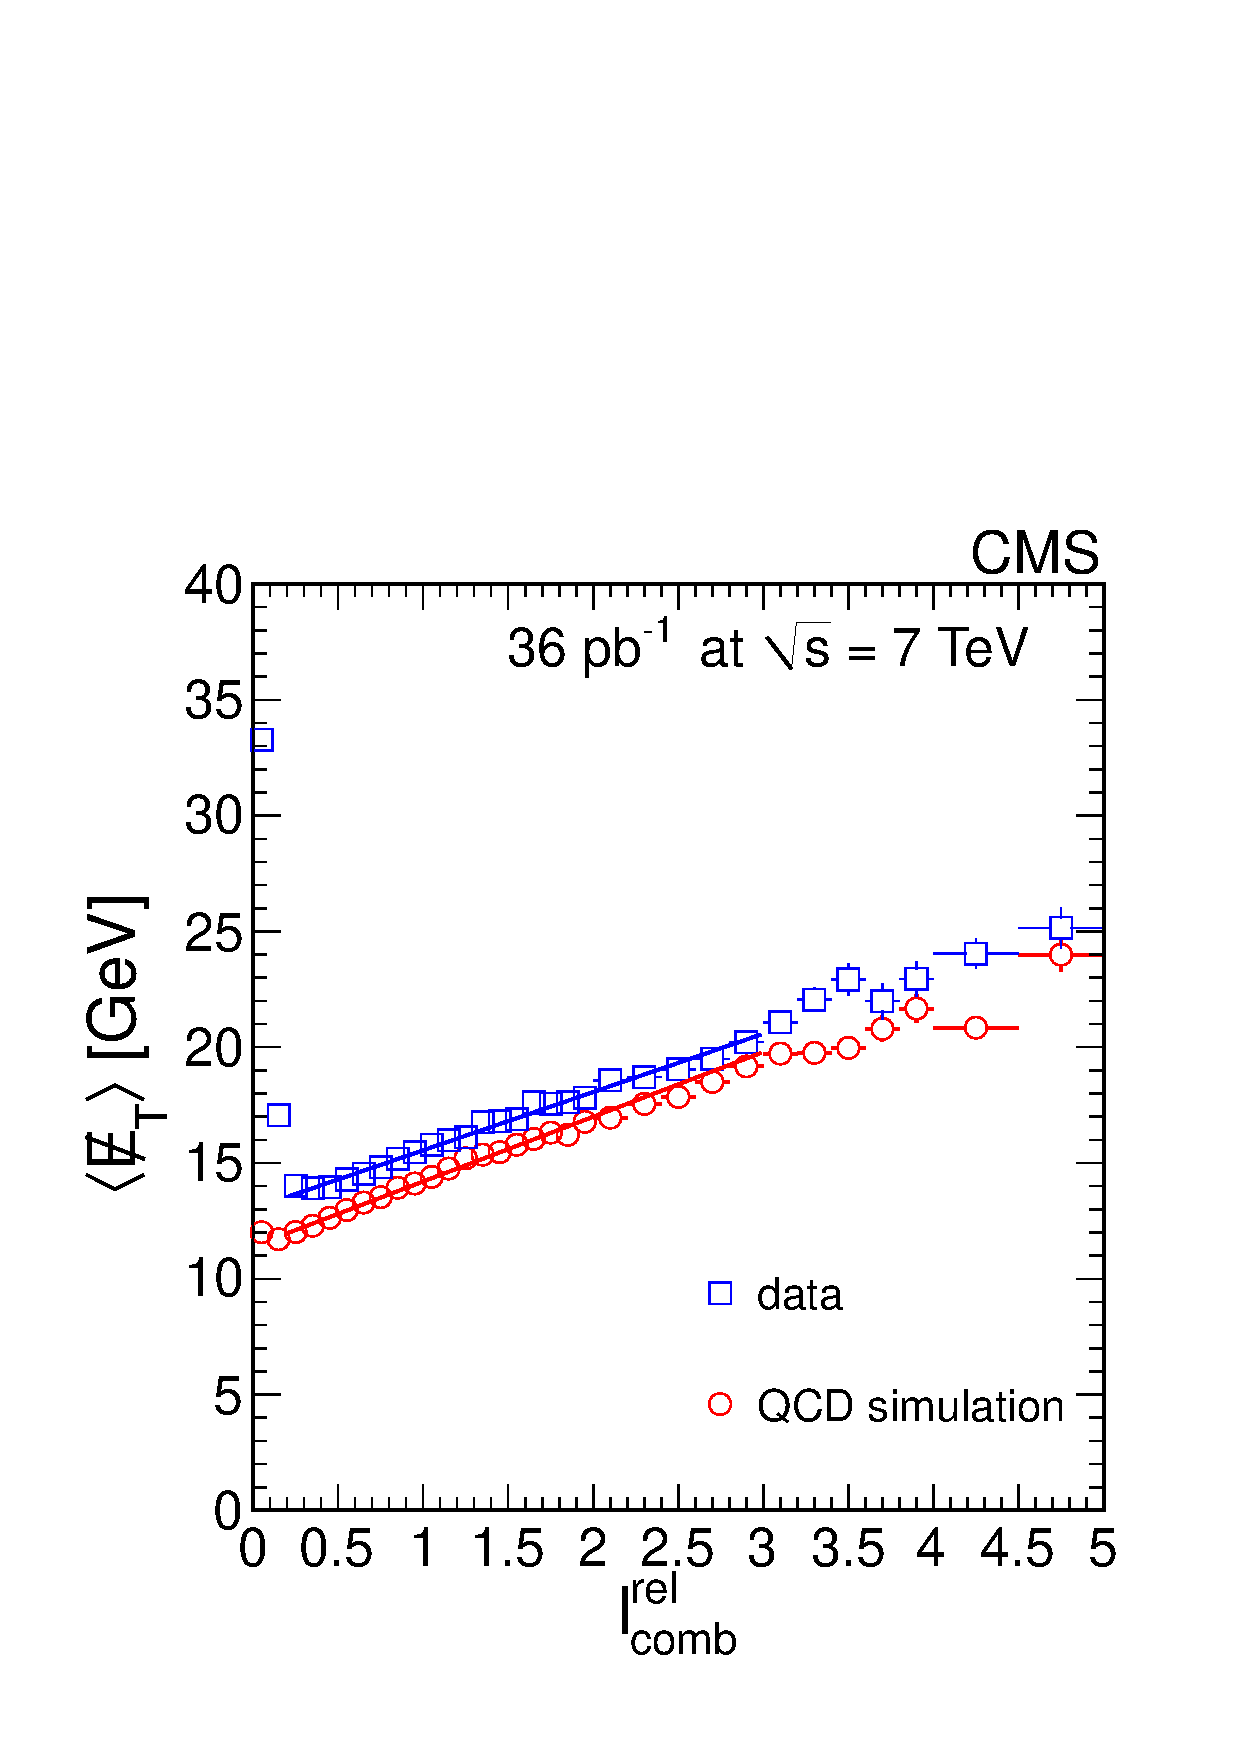
\includegraphics[width=7.5cm]{figs/Wmn_METvsIso.pdf}
    \caption{Left: distribution of the corrected $\MET$ for selected events
with a non isolated muon (black points) superimposed
on the distribution of uncorrected $\MET$ for the same events (blue, dashed line) and
$\MET$ for events with an isolated muon (black, solid histogram). All distributions are from simulated QCD events.
The shaded area represents the systematic uncertainty due to corrections
with factors $\alpha \pm \Delta \alpha$, for $\Delta \alpha = 0.08$.
Right: distribution of the average $\MET$ versus $\IRelComb$
for simulated QCD events (red circles) and
for data (blue squares).
The high values of $\MET$ in the first two bins in $\IRelComb$
are due to the presence of the W signal events. The superimposed lines are linear fits
in the range $[0.2, 3.0]$ of $\IRelComb$.
    \label{figure:Wmunu_QCD}}
}
\end{figure}
\begin{figure}[htbp]
{\centering
    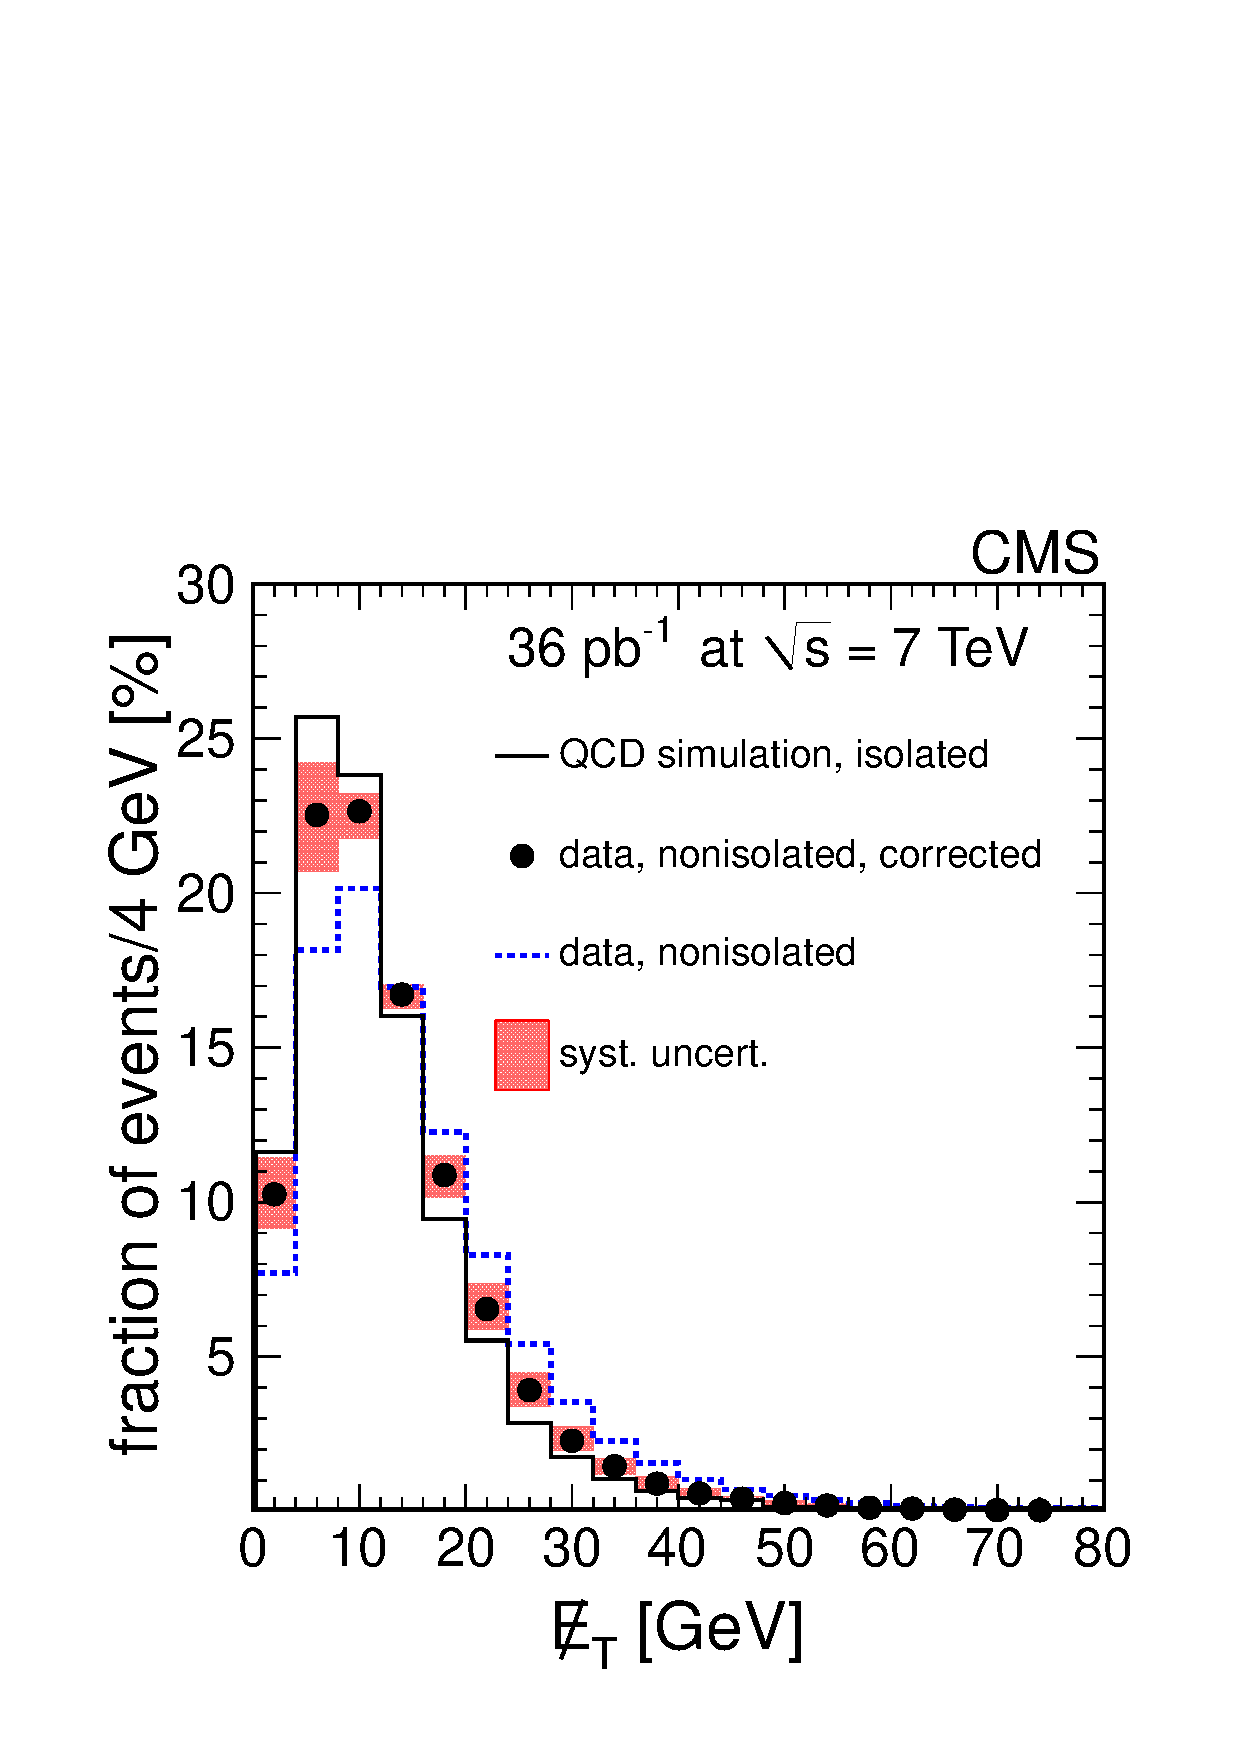
\includegraphics[width=7.5cm]{figs/qcd_template.pdf}
    \caption{
Distribution of the corrected $\MET$ for selected events
with a nonisolated muon in data (black points) superimposed
on the uncorrected $\MET$ distributions for data (blue dashed line) and
simulated QCD events (black, solid histogram, same as
the black, solid histogram in Fig.~\ref{figure:Wmunu_QCD}).
The shaded area represents the systematic uncertainty due to corrections with factors
$\alpha \pm \Delta \alpha$ for $\Delta \alpha = 0.08$.
    \label{figure:Wmunu_QCD_data}}
}
\end{figure}

The same positive correlation between $\MET$ and $\IRelComb$ is observed in the data
(blue squares in Fig.~\ref{figure:Wmunu_QCD}, right).
A correction $\MET^\prime = \MET/(1+\alpha\,\IRelComb)$, with $\alpha \approx 0.2$,
was applied.
The shapes obtained in data are shown in Fig.~\ref{figure:Wmunu_QCD_data} where
the uncorrected and corrected data shapes from events selected by inverting the isolation requirement, together with the
simulation expectation for events with an isolated muon, are shown.
The shaded area in Fig.~\ref{figure:Wmunu_QCD_data} is bounded by the two distributions, obtained using two extreme correction
parameters $\alpha \pm \Delta \alpha$, with $\Delta \alpha = 0.08$, as evaluated in simulations.
This area is taken as a systematic uncertainty on the QCD background shape.

Several parameterizations for the correction are considered,
but the impact on the corrected distribution and therefore on the final result is small.
Associated uncertainties on the cross section and ratios are evaluated as the differences between
the fit results obtained with the optimal $\alpha$ value and
two extreme cases, $\alpha \pm \Delta \alpha$.


The following signal yields are obtained: $140\,757 \pm 383$ for the inclusive sample,
$56\,666\pm240$ for the $\Wmmn$ sample, and $84\,091\pm291$ for the $\Wpmn$ sample.

The $\MET$ distributions are presented in
Fig.~\ref{figure:Wmunu_exp_fit} (full sample) and Fig.~\ref{figure:Wmn_PlusMinus}
 (samples selected by the muon charge) superimposed on the individual fitted
contributions of the W signal and the EWK and QCD backgrounds.
Figures~\ref{figure:Wmunu_exp_fit} and~\ref{figure:Wmn_PlusMinus}
show the $\MET$ distributions for data and fitted signal, plus background components.
 Figure~\ref{figure:Wmunu_exp_fit_mt}
% and~\ref{figure:Wmn_PlusMinus_mt}
shows the $\MT$ distributions for data and signal, plus background components, fitted
from the $\MET$ spectra.

% The fitted W parameters are summarized in Tables~\ref{table:Wmunu_tot_xs}
% for the two choices of fit parameters. The error shown is only statistical.
 \begin{figure}[!ht] {\centering
   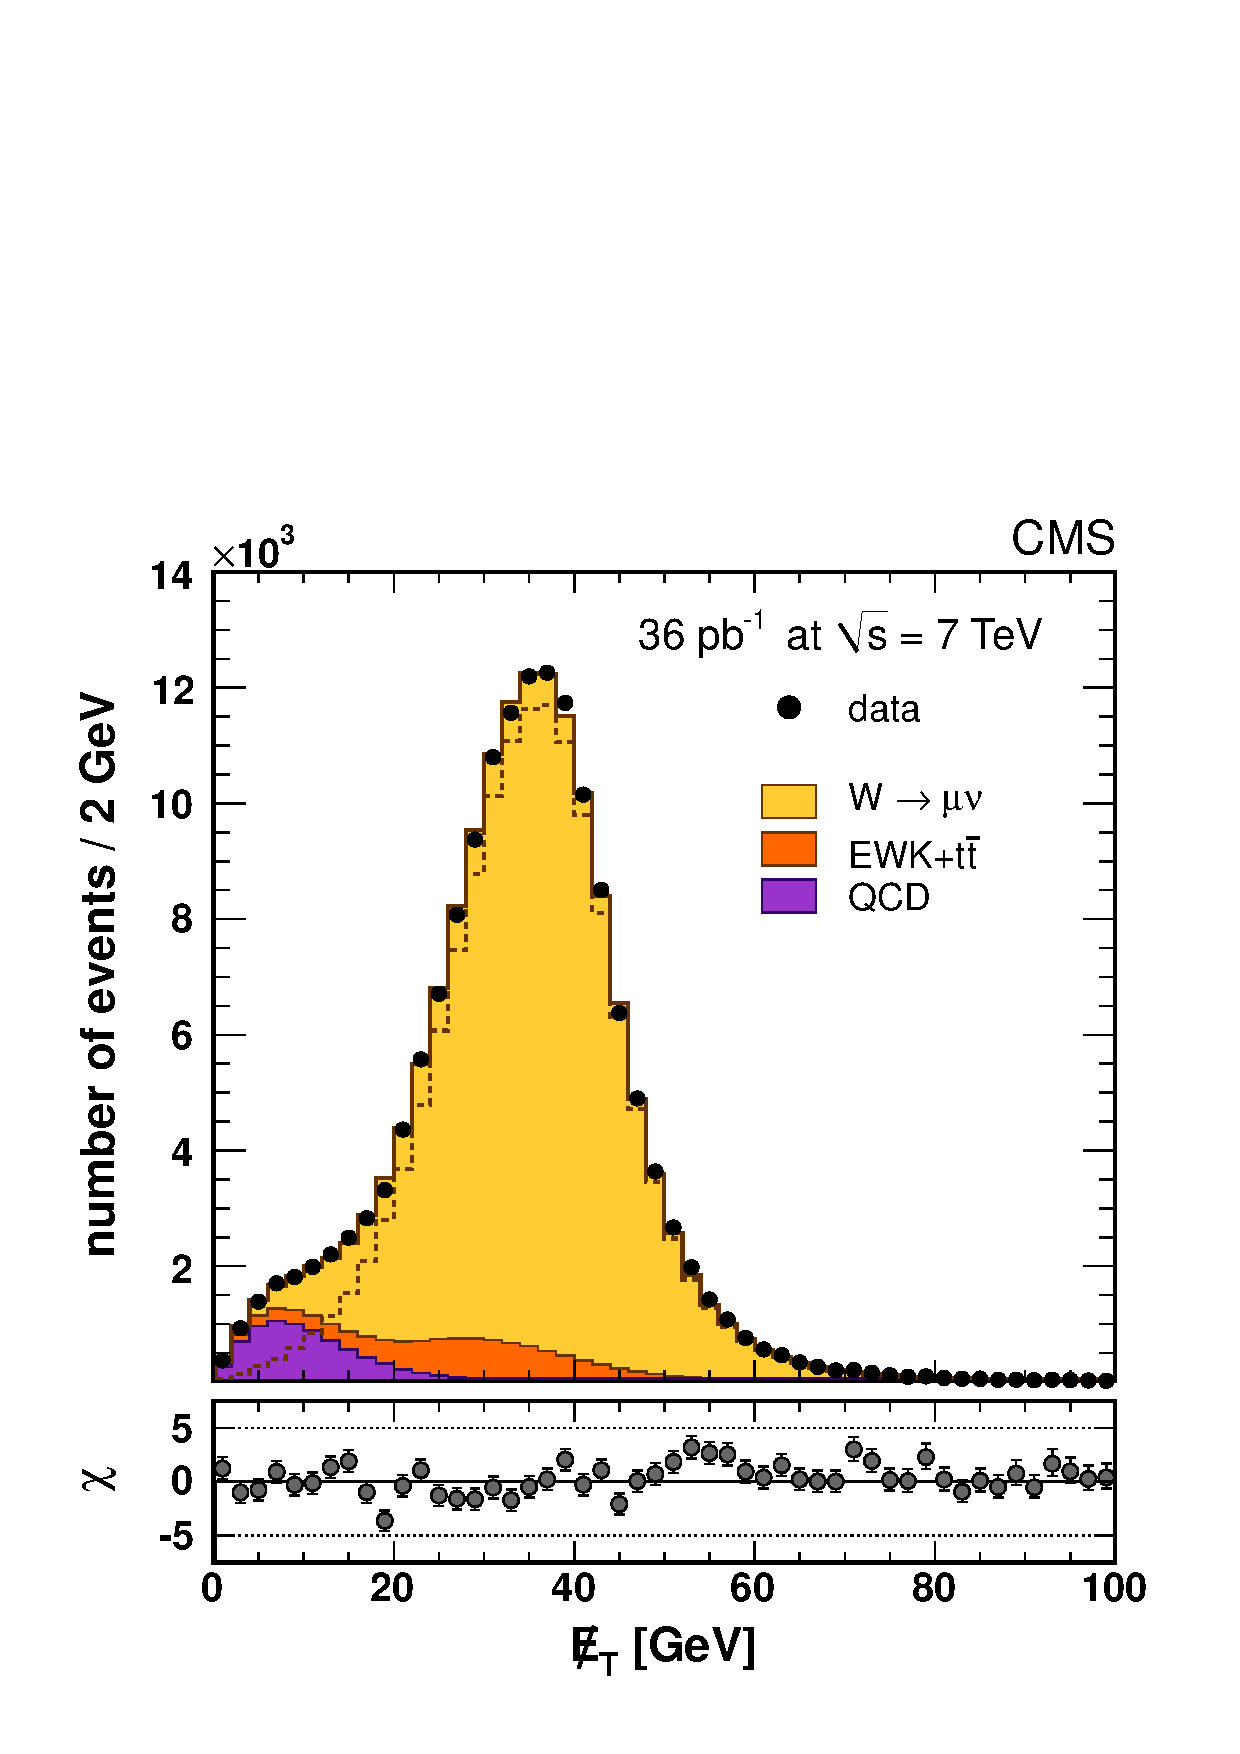
\includegraphics[width=7cm]{figs/Wmn_MET.pdf}
   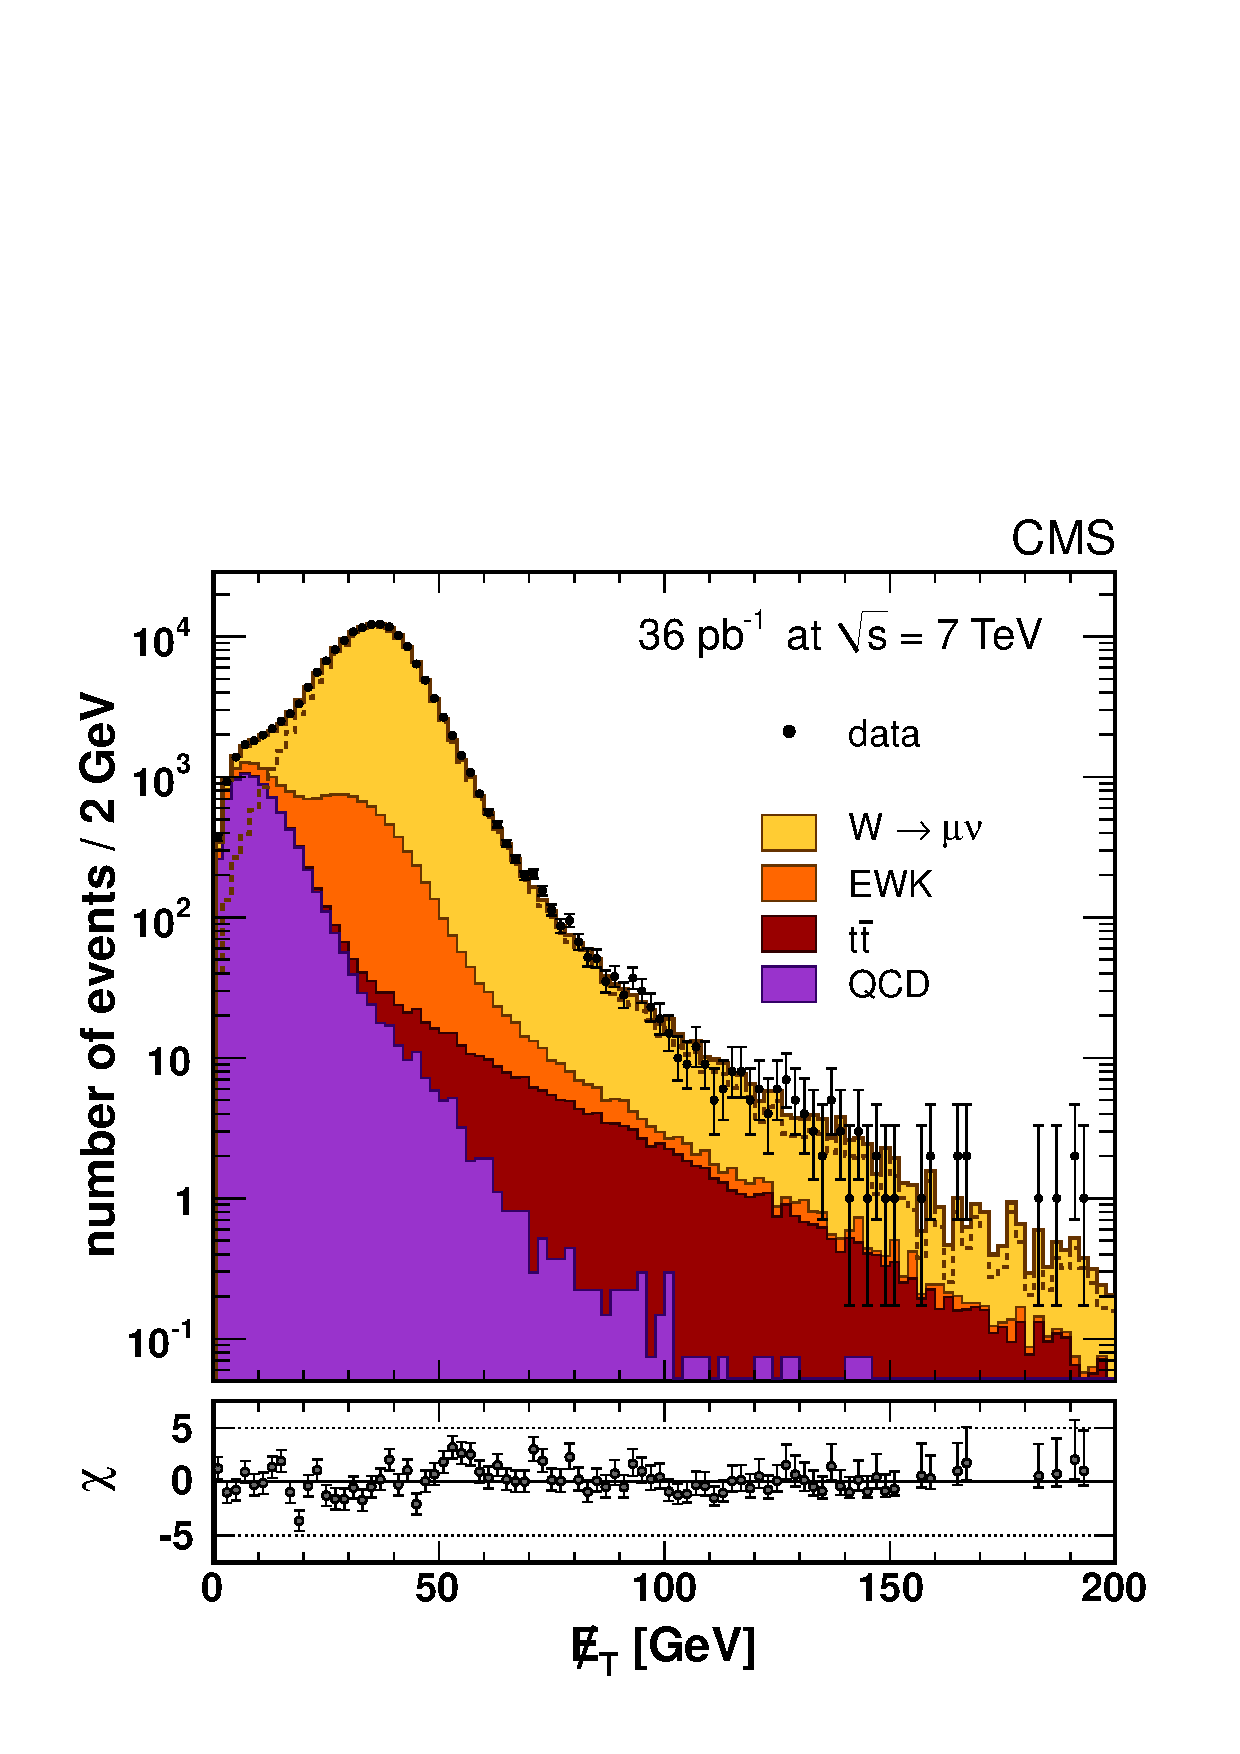
\includegraphics[width=7cm]{figs/Wmn_MET_log.pdf}
     \caption{
The $\MET$ distribution for the selected $\Wmn$ candidates on
a linear scale (left) and on a logarithmic scale (right).
The points with the error bars represent the data. Superimposed are the
contributions obtained with the fit
for QCD background (violet, dark histogram), all other backgrounds
(orange, medium histogram), and signal plus  background (yellow, light histogram).
The black dashed line is the fitted signal contribution.
     \label{figure:Wmunu_exp_fit}}
}
 \end{figure}

\begin{figure}[!ht] {\centering
   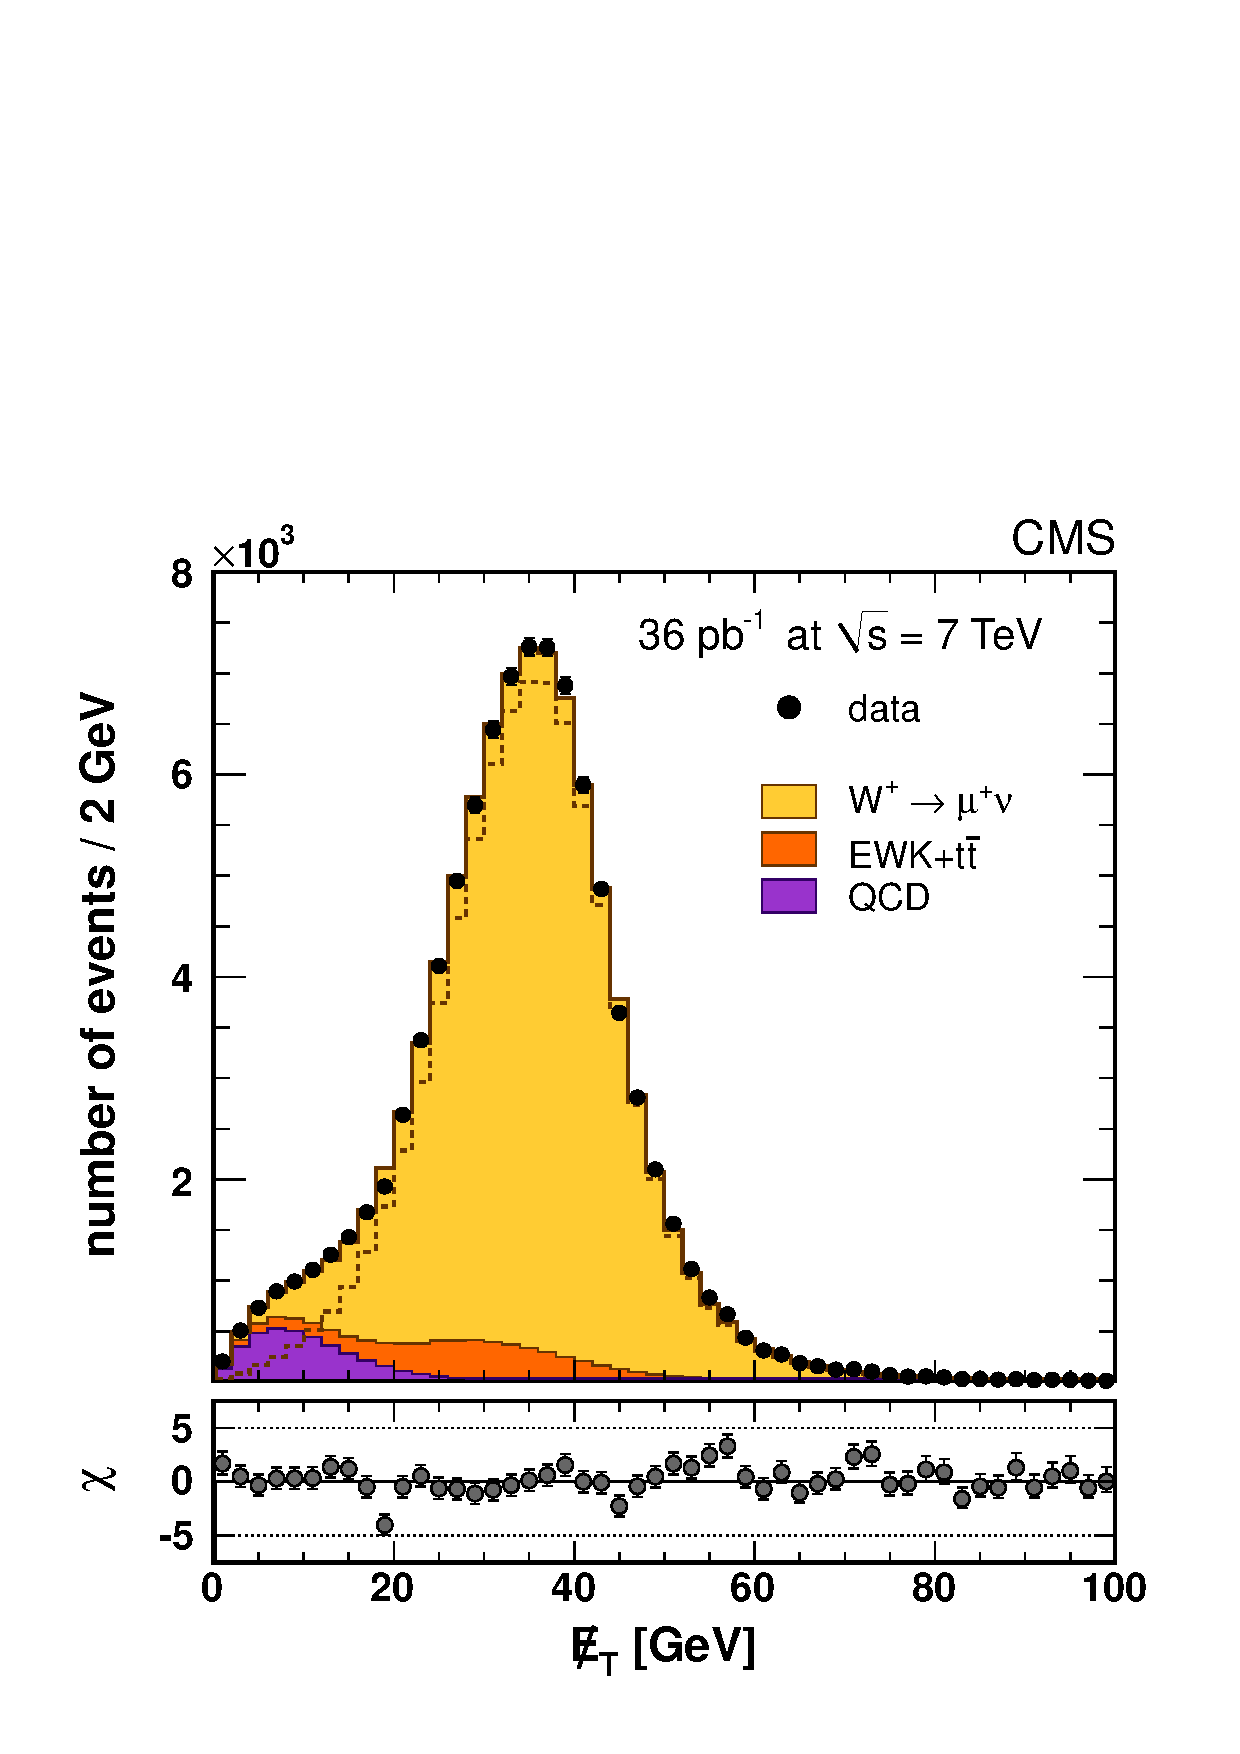
\includegraphics[width=7cm]{figs/Wmn_MET_plus.pdf}
   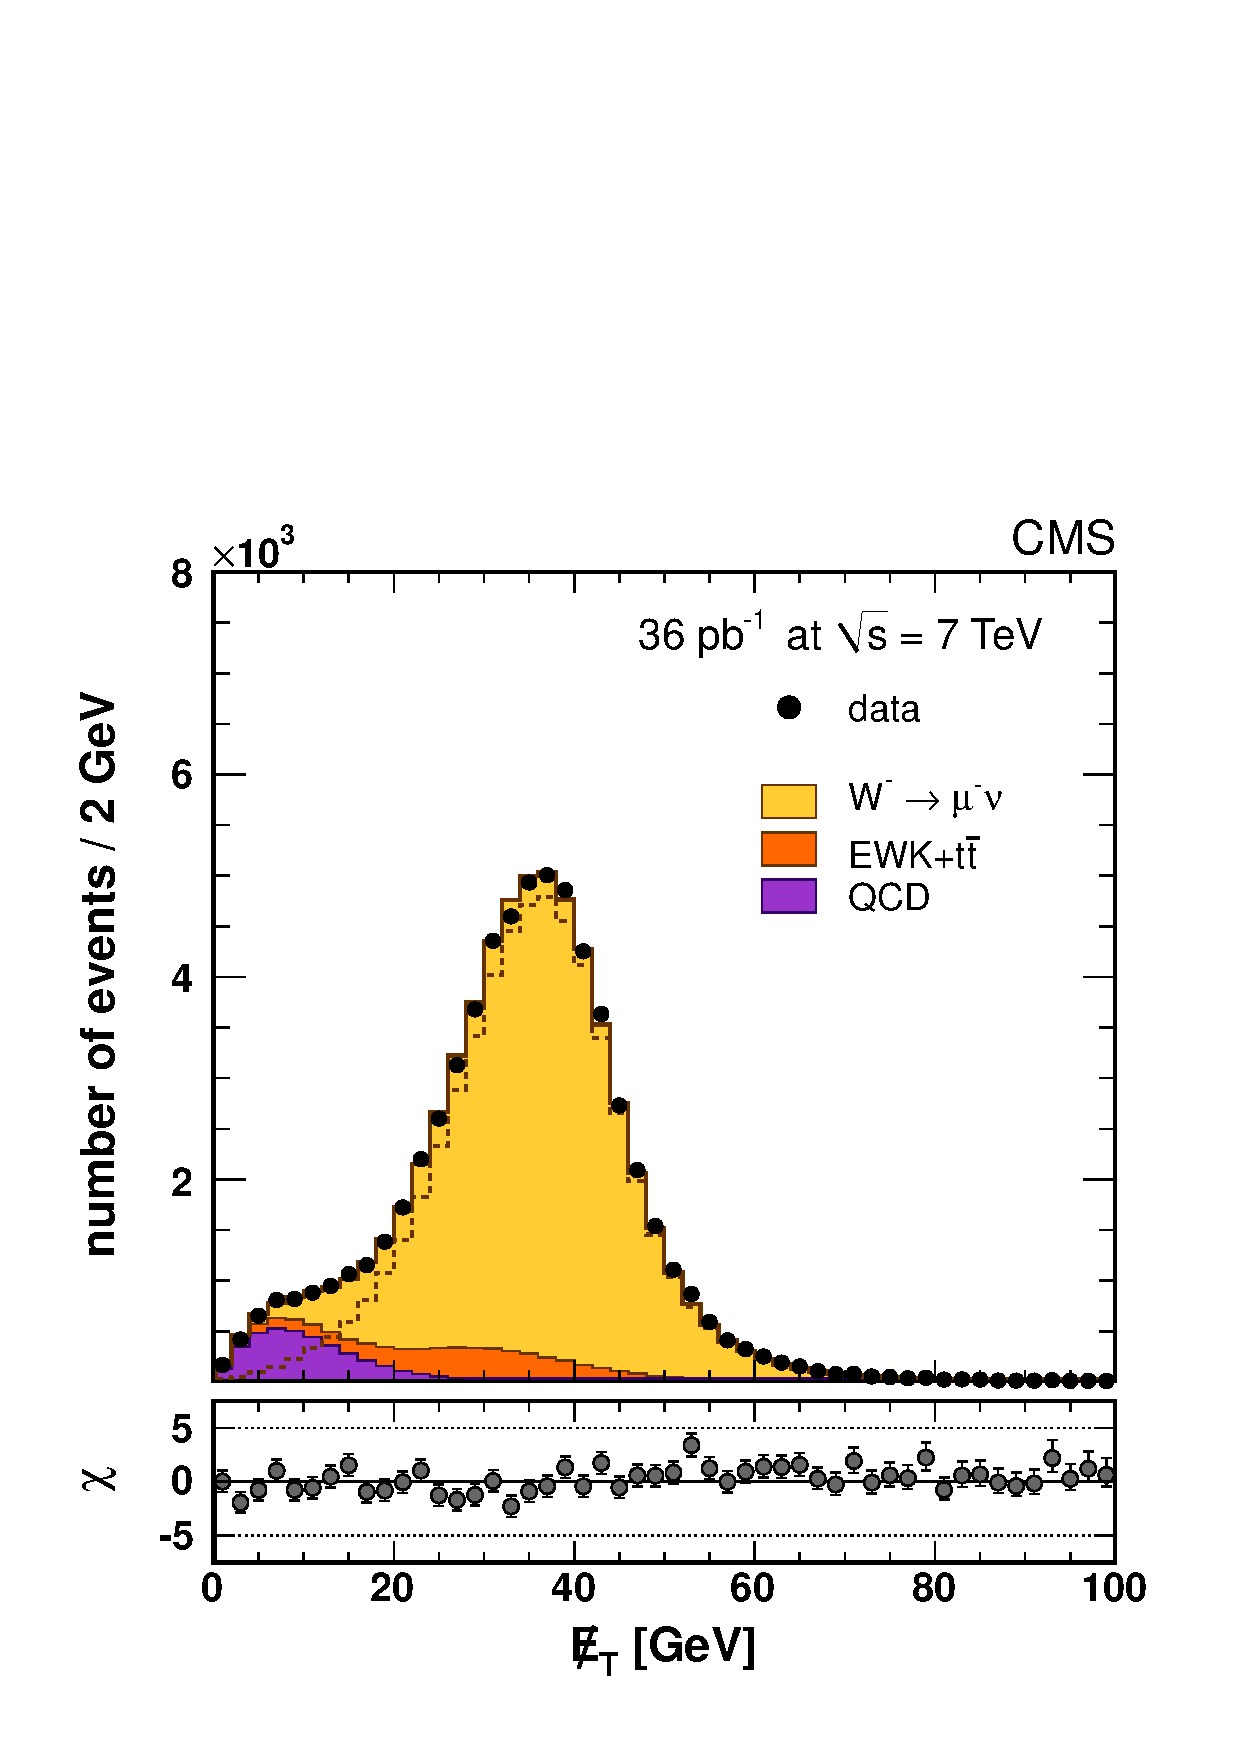
\includegraphics[width=7cm]{figs/Wmn_MET_minus.pdf}
    \caption{
The $\MET$ distributions for the selected W$^+$ (left) and W$^-$ (right) candidates.
The points with the error bars represent the data. Superimposed are the contributions
obtained with the fit for QCD background (violet, dark histogram), all other backgrounds
(orange, medium histogram), and signal plus background (yellow, light histogram).
The black dashed line is the fitted signal contribution.
    \label{figure:Wmn_PlusMinus}}
}
\end{figure}

 \begin{figure}[!ht] {\centering
   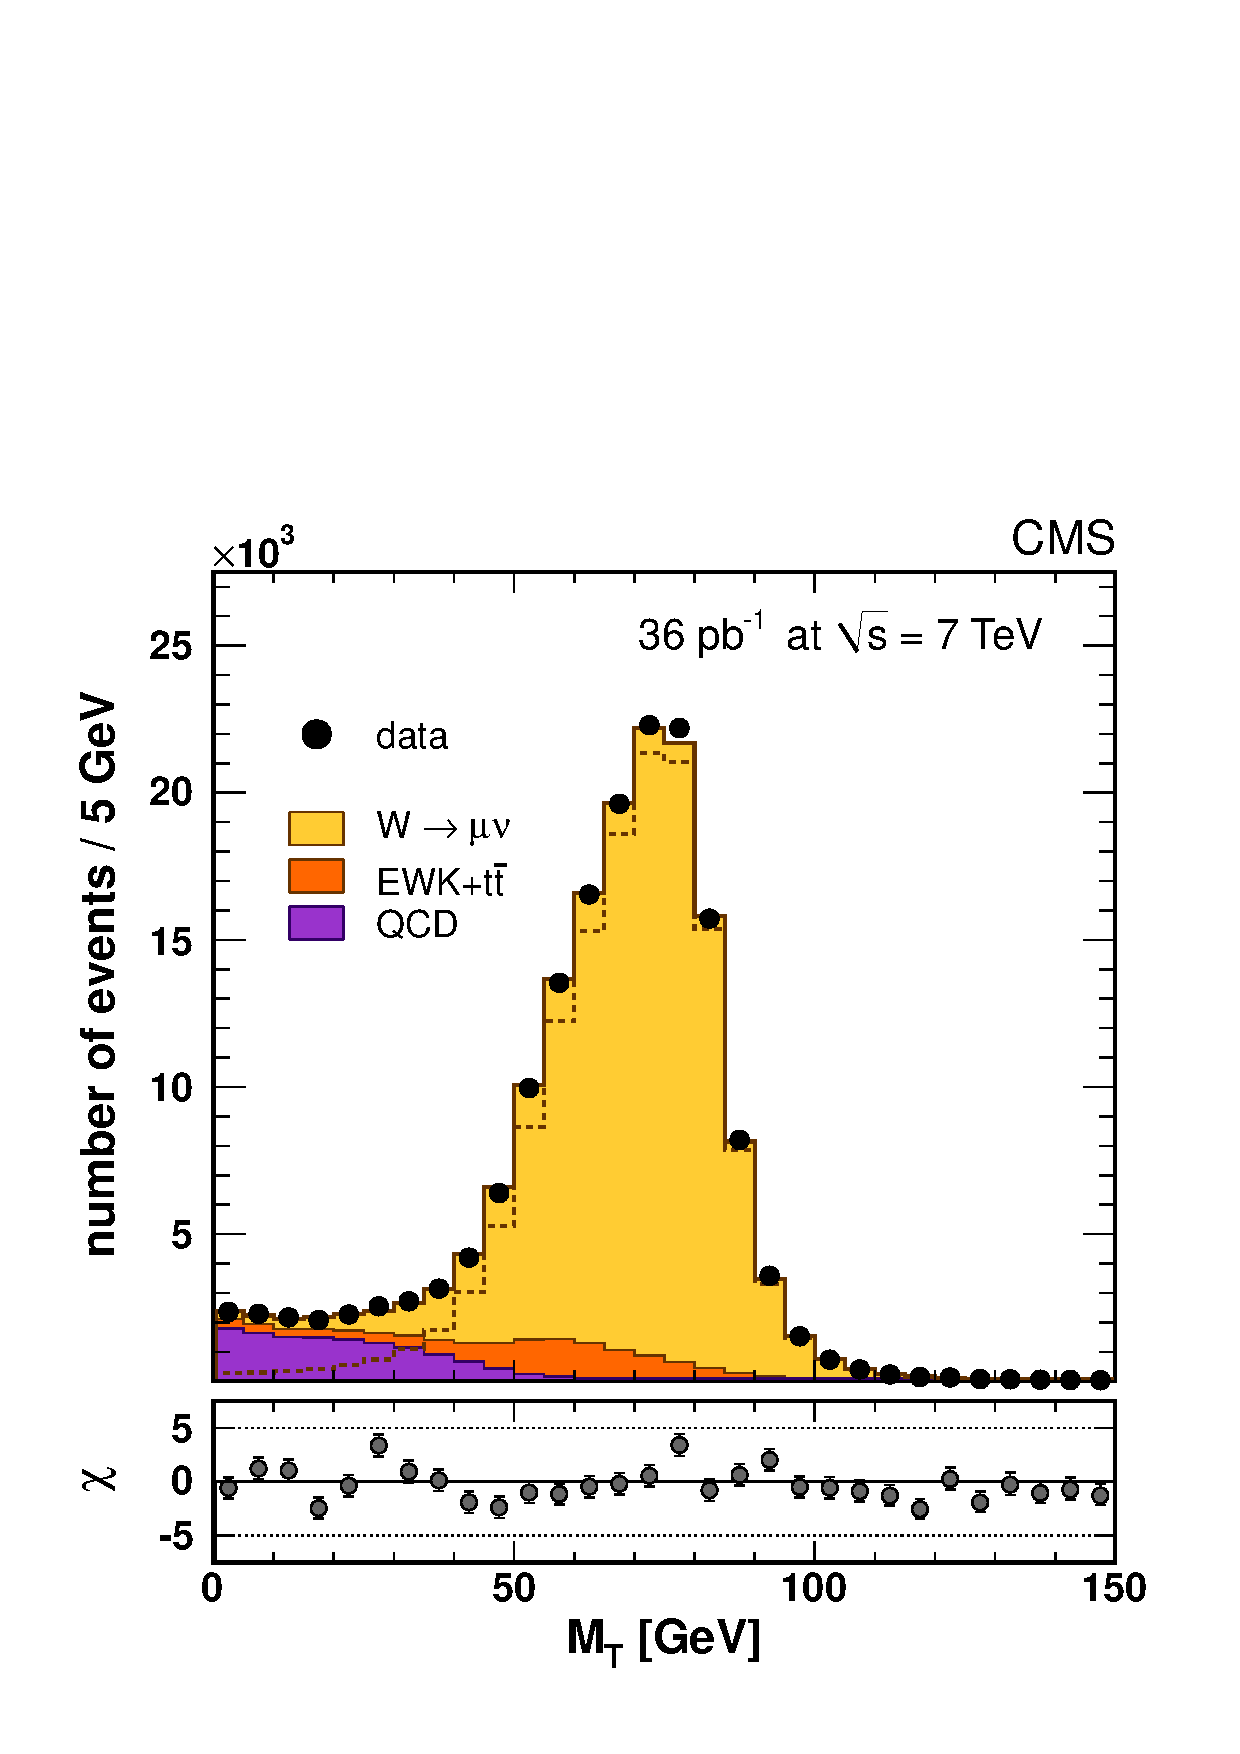
\includegraphics[width=7cm]{figs/Wmn_MT.pdf}
   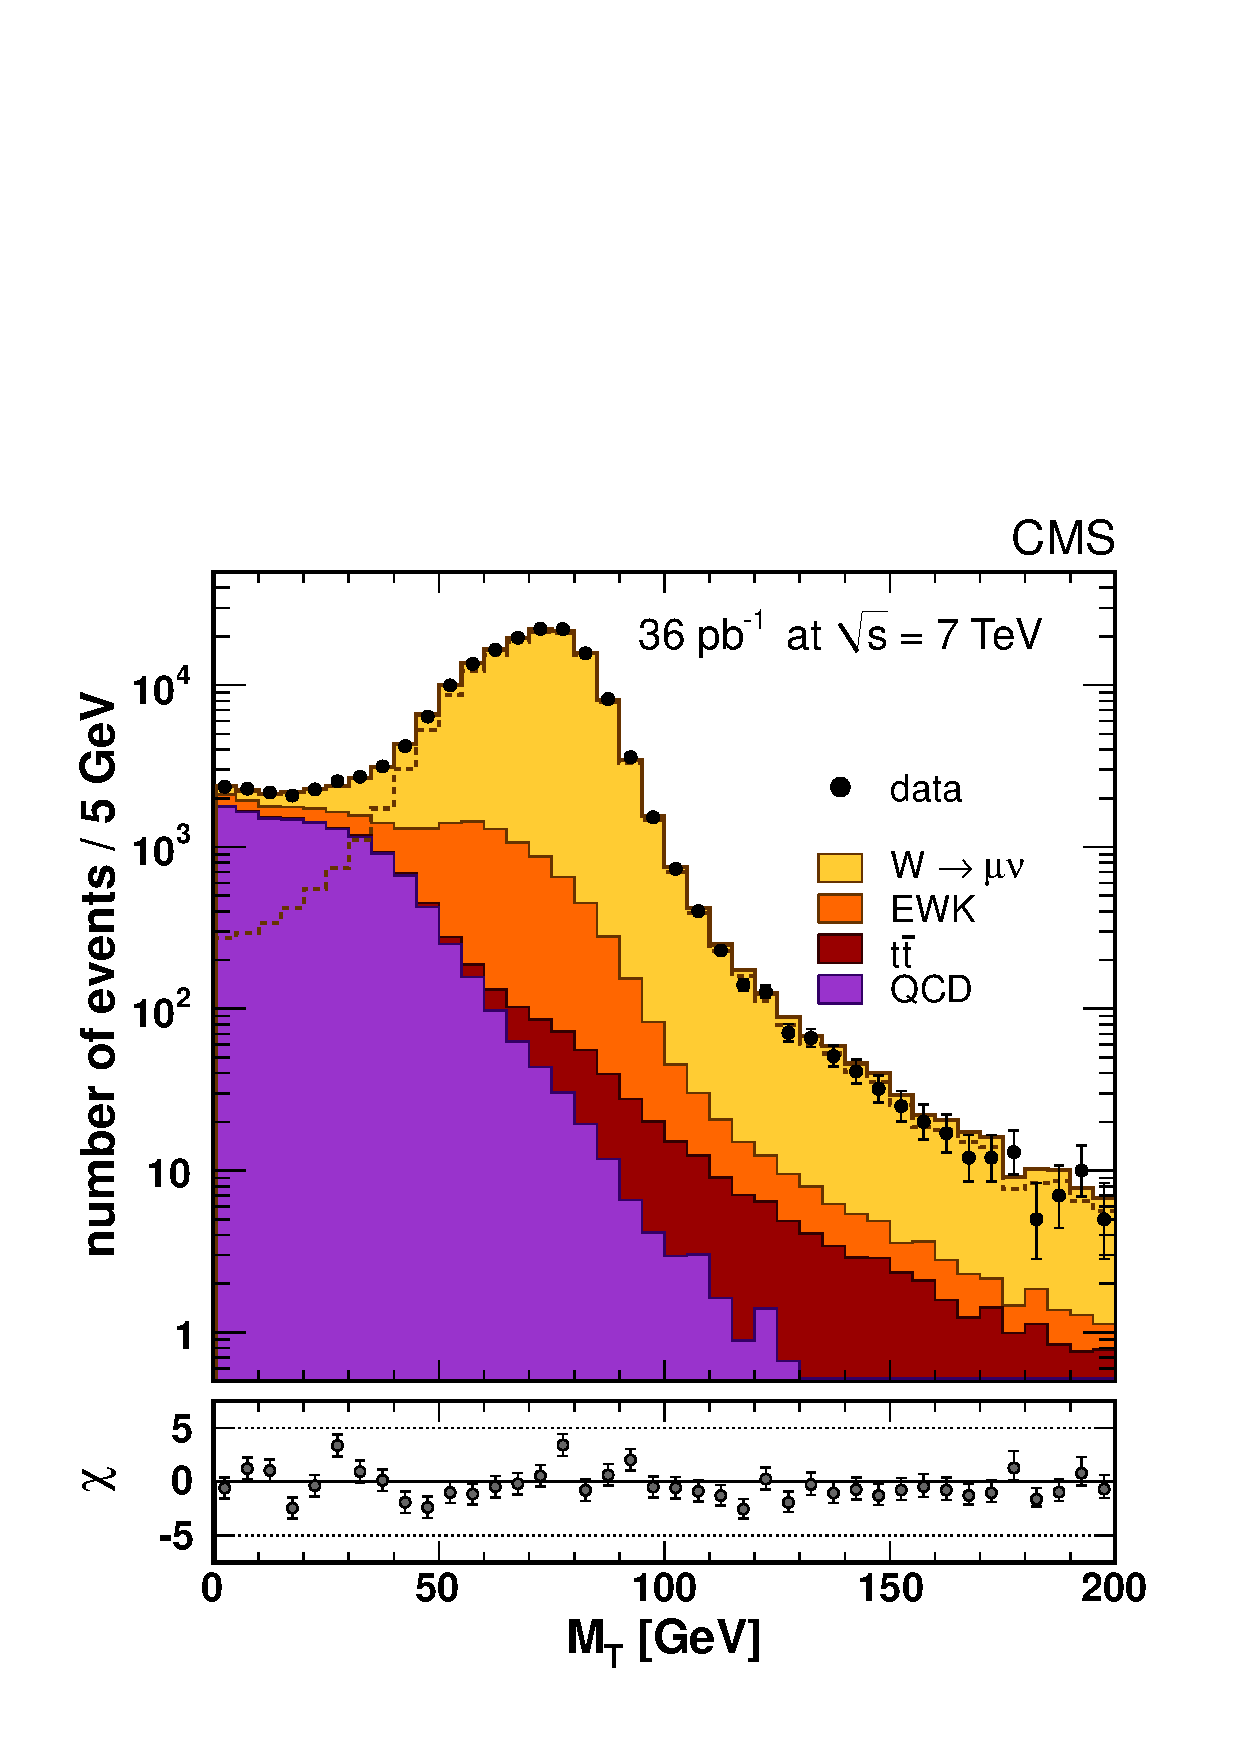
\includegraphics[width=7cm]{figs/Wmn_MT_log.pdf}
     \caption{
The $\MT$ distribution for the selected $\Wmn$ candidates on
a linear scale (left) and on a logarithmic scale (right).
The points with the error bars represent the data. Superimposed are the
contributions obtained with the fit
for QCD background (violet, dark histogram), all other backgrounds
(orange, medium histogram), and signal plus background (yellow, light histogram).
The black dashed line is the fitted signal contribution.
     \label{figure:Wmunu_exp_fit_mt}}
}
 \end{figure}
